\chapter{Method}
\label{chap:method}
Describe earlier approach:

Rule based v(s,o) matching

How this led to trying more generalizable approaches:

Describe current process:

dependency parsing gigacorpus to ldh, xdh, xdx formats;

(gigacorpus info -- did I use full corpus or sample? check)

same for PDT responses;

dependency-based tf-idf for responses vs. gigacorpus;

get sorted superset of XGS \& response terms and their tf-idf scores;

get cosine of these vectors (``TC'' for tf-idf cosine; discuss how this compares to recent encoder based approaches (BERT), as this essentially is a primitive, more transparent encoder);

rank responses by TC;

get spearman of XGS \& TC based ranking vs ranking via the weighted feature annotations.

\section{Introduction}
The method used to analyze PDT responses throughout this dissertation represents an evolution from my own earlier attempts. In this chapter, I summarize my previous work and explain the current method.

%%%% BEGIN material from Qual Paper (BEA 2013) %%%%
\section{First approaches: Rule based semantic triple matching}
This section summarizes relevant work first presented in \citet{king:dickinson:13} and \citet{king:dickinson:14}; please see those papers for deeper discussion. Like the current research, my previous work focused on analyzing non-native speaker (NNS) responses to a picture description task (PDT) by comparison with native speaker (NS) responses. I did not know a priori if such a task would be within range for a single researcher using off the shelf tools, so my initial work sought to uncover challenges and determine whether variation in the form and content of responses could be manageable.

%Research in SLA often
%relies on the ability of task design to induce particular linguistic
%behavior \citep{skehan1998assessing}, and the PDT should induce
%interactive behavior.  Moreover, the use of the PDT as a reliable
%language research tool is well-established in areas of study ranging
%from SLA to Alzheimer's disease \citep{ellis2000task,
%  forbes2005detecting}.

%The NNSs were intermediate and upper-level adult English learners in
%an intensive English as a Second Language program at Indiana
%University. We rely on visual stimuli here for a number of
%reasons. Firstly, computer games tend to be highly visual, so
%collecting responses to visual prompts is in keeping with the nature
%of our desired ILT. Secondly, by using images, the information the
%response should contain is limited to the information contained in the
%image. Relatedly, particularly simple images should restrict elicited
%responses to a tight range of expected contents.
%

I knew this would require some constraint of the responses, and without a readily available and appropriate dataset for the task, I crafted my own small PDT and collected a small corpus of NS and NNS responses. I also expected to rely on some kind of rule based approach for extracting \textit{verb(subject,object)} triples from syntactic dependency parses. Thus, for this initial experiment, I chose or developed each of the visual stimuli because
it presents an event that I believe to be transitive in nature and
likely to elicit responses with an unambiguous subject, verb and
object, thereby imposing some restrictions on form and content.

\begin{figure}[htb!]
%[width=0.8\columnwidth]
\begin{center}
\begin{tabular}{|c|}
\hline
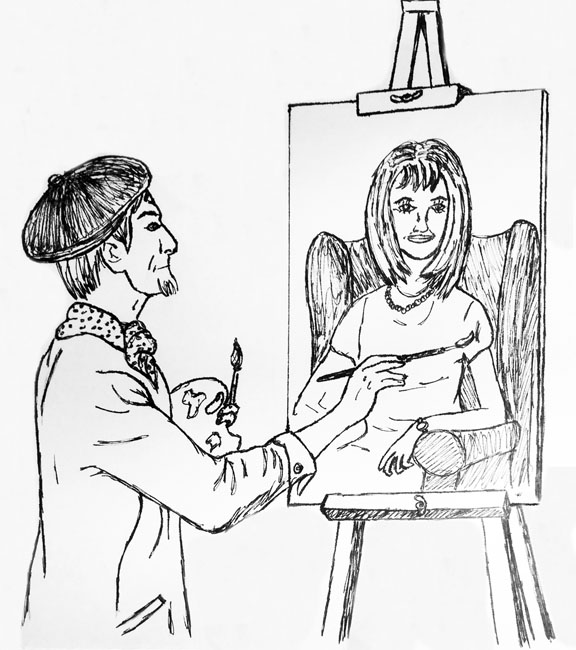
\includegraphics[width=0.8\columnwidth]{figures/exampleprompt.jpg}\\
\hline
\textbf{Response (L1)} \\
\hline
He is droning his wife pitcher. (Arabic)\\
\hline
The artist is drawing a pretty women. (Chinese) \\
\hline
The artist is painting a portrait of a lady. (English) \\
\hline
The painter is painting a woman's paint. (Spanish)\\
\hline
\end{tabular}
\end{center}
\caption{Example item and NNS responses}
\label{fig:example-picture}
\end{figure}

The PDT consists of 10 items (8 line drawings and 2 photographs) intended to elicit a single sentence each; an example is given in Figure~\ref{fig:example-picture}. Participants
were asked to view the image and describe the action in either past or present tense. Responses were typed by the participants themselves in a computer lab with spell checking disabled.
I collected responses from 53
informants (14 NSs, 39 NNSs), for a total of 530 sentences. 
\subsection{Method}
\label{sec:method}

My process in this initial work was to parse a NNS sentence into a dependency representation
(section~\ref{sec:syntactic-form})
and then extract a simple semantic
form from this parse
(section~\ref{sec:semantic-form})
to compare to
gold standard semantic forms similarly derived from the NS responses.

\subsection{Obtaining a syntactic representation}
\label{sec:syntactic-form}
Because dependency parsing focuses on identifying dependency
relations, rather than constituents or phrase structure, it clearly
labels the subject, verb and object of a sentence, which can then map
to a semantic form \citep{Kuebler.McDonald.Nivre-09}. In these experiments, I took a na\"ive approach in which subject, verb and
object were considered sufficient for deciding whether or not a
response accurately describes the visual prompt.

As in my current research, I used the Stanford Parser for this task, trained on the Penn Treebank 
\citep{demarneffe:ea:06, 
klein:manning:03}.\footnote{\url{http://nlp.stanford.edu/software/lex-parser.shtml}} 
%
Using the parser's options, I set the output to be Stanford typed
dependencies, a set of labels for dependency relations. The Stanford
parser has a variety of options for the specific
ouput, e.g., how one wishes to treat prepositions
\citep{defmarneffe:manning:12}.  I used only two non-default parser options ({\tt
  CCPropagatedDependencies} and {\tt CCprocessed}\footnote{\url{http://nlp.stanford.edu/software/dependencies_manual.pdf}}) in order to:
%
1) omit prepositions and conjunctions from the sentence text and
instead add the word to the dependency label between content words;
and 2) propagate relations across conjunctions.  These decisions
are important to consider for any semantically-informed processing of
learner language.

To see the impetus for removing prepositions, consider the learner
example in Figure~\ref{fig:prep-dependency}, where the preposition \textit{with} is
relatively unimportant to collecting the meaning.  Additionally,
learners often omit, insert, or otherwise use the wrong preposition
\citep{chodorow:et:al:07}.  The default parser would present a
\texttt{prep} relation between \textit{played} and \textit{with},
obscuring what the object is; with the options set as above, however,
the dependency representation folds the preposition into the label
(\texttt{prep\_with}), instead of keeping it in the parsed string, as
shown in Figure~\ref{fig:prep-dependency}.

\begin{figure}[htb!]
\begin{center}
    \begin{dependency}[arc edge,text only label,label style={above}]
    \begin{deptext}[column sep=.5em]
      \textit{vroot} \& The \&[1em] boy \&[1em] played \& with \& a \&[1em] ball \\
    \end{deptext}
    \depedge{4}{3}{nsubj}
    \depedge[arc angle=90]{1}{4}{root}
    \depedge{4}{7}{prep\_with}
%    \depedge[arc angle=35,edge style={dotted}]{7}{6}{det}
%    \depedge[edge style={dotted}]{3}{2}{det}
    \depedge[arc angle=35]{7}{6}{det}
    \depedge{3}{2}{det}
  \end{dependency}
\end{center}
\caption{Dependency parse showing collapsed preposition dependencies.}
\label{fig:prep-dependency}
\end{figure}

This is a lenient approach to prepositions, as prepositions
are not without semantic meaning---e.g., \textit{the boy played in a
  ball} means something quite different from the \textit{with} example.  However, this option makes it moderately easier to compare the meaning to an expected semantic form (e.g., \textit{play(boy,ball)}).

As for propagating relations across conjunctions, this also simplifies the representation somewhat and makes it easier to connect verbs and their arguments, as needed for the semantic
form used in comparisons. For a conjunction like \textit{cats and dogs}, for example, the default settings would produce \texttt{cc(cats, and)} and \texttt{conj(cats, dogs)}, but the chosen settings would collapse this into \texttt{conj\_and(cats, dogs)}, omitting the dependency that merely labels a conjunction relation between the first conjunct and the conjunction.

Given the rule based approach to matching \textit{verb(subject,object)} triples, many dependency relations are irrelevant for the next step of obtaining a semantic form.  For example, in this work I ignored determiner (\texttt{det}) relations between a noun and its determiner, allowing for variability in how a learner produces
noun phrases. 

\subsection{Obtaining a semantic representation}
\label{sec:semantic-form}

\subsubsection{Sentence types}

\begin{table*}[htb!]
\begin{center}
\begin{tabular}{|c|l|l|r|r|}
\hline
Type & Description & Example & NS & NNS \\
\hline
 A & Simple declarative transitive & The boy is kicking the ball. & 117 & 286 \\
 \hline
 B & Simple + preposition & The boy played with a ball. & 5 & 23 \\
 \hline
 C & Missing tensed verb & Girl driving bicycle. & 10 & 44 \\
 \hline
 D & Missing tensed verb + preposition & Boy playing with a ball. & 0 & 1 \\
 \hline
 E & Intransitive (No object) & A woman is cycling. & 2 & 21 \\
 \hline
 F1 & Passive & An apple is being cut. & 4 & 2 \\
 \hline
 F2 & Passive with agent & A bird is shot by a man. & 0 & 6 \\
 \hline
 Ax & Existential version of A or C & There is a boy kicking a ball. & 0 & 0 \\
 \hline
 Bx & Existential version of B  or D & There was a boy playing with a ball. & 0 & 0 \\
 \hline
 Ex & Existential version of E & There is a woman cycling. & 0 & 0 \\
 \hline
 F1x & Existential version of F1 & There is an apple being cut. & 0 & 1 \\
 \hline
 F2x & Existential version of F2 & There is a bird being shot by a man. & 0 & 0 \\
 \hline
 Z & All other forms & The man is trying to hunt a bird. & 2 & 6 \\
 \hline
\end{tabular}
\end{center}
\caption{Sentence type examples, with distributions of types for
  native speakers (NS) and non-native speakers (NNS)}
\label{tab:sentence-type}
\end{table*}

I categorized the sentences in the corpus into 12 types, shown in
Table~\ref{tab:sentence-type}. I established these types because each
type corresponds to a basic sentence structure and thus has consistent
syntactic features, leading to predictable patterns in the dependency
parses.
%We discuss the distribution of sentence types in
%section~\ref{sec:sentence-distribution}.

\subsubsection{Rules for sentence types}


A sentence type indicates that the subject,
verb, and object can be found in a particular place in the parse,
e.g., under a particular dependency label.
For example, for simple transitive sentences of type A,
the words labeled {\tt nsubj}, {\tt root}, and {\tt dobj} exactly
pinpoint the necessary information.
Thus, the patterns for extracting semantic information---in the form
of \textit{verb(subj,obj)} triples---reference particular Stanford
typed dependency labels, part-of-speech (POS) tags, and interactions
with word indices.

More complicated sentences or those containing common learner errors
(e.g., omission of the copula \textit{be}) required slightly more
complicated extraction rules, but, since this work examined only transitive
verbs, these still boiled down to identifying the
sentence type and extracting the appropriate triple.  This was accomplished by
arranging a small set of binary features into a decision tree to
determine the sentence type, as shown in
Figure~\ref{fig:decision-tree}.


\begin{figure*}[htb!]
\begin{center}
\begin{tikzpicture}
\tikzset{level distance=3.5em}
\tikzset{edge from parent/.append style={->}}
\Tree
[.{\tt expl}?
  \edge node[auto=right,pos=.6,inner sep=1pt]{Y};
  [.{\tt auxpass}? 
  	\edge node[auto=right,pos=.6,inner sep=1pt]{Y};
  	[.{\tt agent}? 
		\edge node[auto=right,pos=.6,inner sep=1pt]{Y};
		[.F2x ]
		\edge node[auto=left,pos=.6,inner sep=1pt]{N};
		[.F1x ]
	]
	\edge node[auto=left,pos=.6,inner sep=1pt]{N};
	[.{\tt dobj}? 
		\edge node[auto=right,pos=.6,inner sep=1pt]{Y};
		[.Ax ]
		\edge node[auto=left,pos=.6,inner sep=1pt]{N};
		[.{\tt prep\_}$\ast$?
			\edge node[auto=right,pos=.6,inner sep=1pt]{Y};
			[.Bx ]
			\edge node[auto=left,pos=.6,inner sep=1pt]{N};
			[.Ex ]
		]
	]
  ]
  \edge node[auto=left,pos=.6,inner sep=1pt]{N};
  [.{\tt nsubjpass}? 
  	\edge node[auto=right,pos=.6,inner sep=1pt]{Y};
  	[.{\tt agent}? 
		\edge node[auto=right,pos=.6,inner sep=1pt]{Y};
		[.F2 ]
		\edge node[auto=left,pos=.6,inner sep=1pt]{N};
		[.F1 ]
	]
	\edge node[auto=left,pos=.6,inner sep=1pt]{N};
	[.{\tt dobj}? 
		\edge node[auto=right,pos=.6,inner sep=1pt]{Y};
		[.{\tt nsubj}?
			\edge node[auto=right,pos=.6,inner sep=1pt]{Y};
			[.A ]
			\edge node[auto=left,pos=.6,inner sep=1pt]{N};
			[.C ]
		]
		\edge node[auto=left,pos=.6,inner sep=1pt]{N};
		[.{\tt nsubj}?
			\edge node[auto=right,pos=.6,inner sep=1pt]{Y};
			[.{\tt prep\_}$\ast$?
			 	\edge node[auto=right,pos=.6,inner sep=1pt]{Y};
				[.B ]
				\edge node[auto=left,pos=.6,inner sep=1pt]{N};
				[.E ]
			]
			\edge node[auto=left,pos=.6,inner sep=1pt]{N};
			[.D ]
			]
		]
	]
  ]
]
\end{tikzpicture}
\end{center}
\caption{Decision tree for determining sentence type and extracting semantic information}
\label{fig:decision-tree}
\end{figure*}

To illustrate, consider the process for the example in Figure~\ref{fig:F2-dependency}.  The
sentence is passed through the parser to obtain the dependency parse shown.
The parsed sentence then moves to the
decision tree shown in Figure~\ref{fig:decision-tree}.
At the top of the tree, the sentence is checked for an {\tt expl}
(expletive) label; having none, it moves rightward to the {\tt
  nsubjpass} (noun subject, passive) node. Because a {\tt
  nsubjpass} label is found, the sentence moves leftward to the {\tt agent}
node. This label is also found, and because the sentence has reached a terminal node, it is labeled as a type F2 sentence.
%
%\begin{exe}
%  \ex\label{ex:F2-type}A bird is shot by a man.
%\end{exe}

\begin{figure}[htb!]
\begin{center}
    \begin{dependency}[arc edge,text only label,label style={above}]
    \begin{deptext}[column sep=.5em]
      \textit{vroot} \& A \& bird \& is \&[2em] shot \& by \& a \&[1em] man \\
    \end{deptext}
    \depedge[arc angle=90]{1}{5}{root}
    \depedge[edge style={dotted}]{3}{2}{det}
    \depedge[arc angle=90]{5}{3}{nsubjpass}
    \depedge[arc angle=30]{5}{4}{auxpass}
    \depedge{5}{8}{agent}
    \depedge[arc angle=40,edge style={dotted}]{8}{7}{det}
  \end{dependency}
\end{center}
\caption{The dependency parse of an example NNS response.}
\label{fig:F2-dependency}
\end{figure}

With the sentence now typed as F2, specific F2 extraction
rules are applied. The logical subject is taken from under the {\tt agent} label,
the verb from {\tt root}, and the logical object from {\tt nsubjpass},
to obtain \textit{shot(man,bird)}, which can be lemmatized to
\textit{shoot(man,bird)}. 
%Very little effort goes into this process:
%the parser is pre-built; the decision tree is small; and the
%extraction rules are minimal.

This much is possible with relatively little effort in part due to the constraints in the
pictures.  For figure~\ref{fig:example-picture}, for example,
\textit{the artist}, \textit{the man in the beret}, and \textit{the
  man} are all acceptable subjects, whereas if there were multiple men
in the picture, \textit{the man} would not be specific enough.
%In future work, we expect to relax such constraints on image contents
%by including rules to handle relative clauses, adjectives and other
%modifiers in order to distinguish between references to similar
%elements, e.g., 
%\textit{a man shooting a bird} vs. \textit{a man reading the
%  newspaper}.

\subsection{Evaluation}
\label{sec:evaluation}

Evaluating this work required addressing two major questions.  First,
how accurately does this approach extract semantic information from potentially
innovative sentences (section~\ref{sec:eval:extraction})?  Due to the
simple structures of the sentences
(section~\ref{sec:sentence-distribution}), this simple system performs moderately well.
Secondly, how many semantic forms does one need in
order to capture the variability in meaning in learner sentences
(section~\ref{sec:eval:coverage})? I operationalized this second
question by asking how well the set of native speaker semantic forms
models a gold standard, with the intuition that a language is largely defined
by native speaker usage, so their answers can serve as targets.  As we
will see, this is a na\"ive view.
\subsection{Basic distribution of sentences}
\label{sec:sentence-distribution}

\begin{table*}[htb!]
\begin{center}
\setlength{\tabcolsep}{.3em}
\begin{tabular}{|l|l|l|cc|r|}
  \hline
  & & Err. type & \multicolumn{2}{c|}{Example} &  \\
  & & (Tot. resp.) & Sentence & Triple & Count (\%)\\
  \hline
  \hline
  \multirow{8}{*}{\begin{sideways}Triple error\end{sideways}} &
  \multirow{4}{*}{\begin{sideways}NNS\end{sideways}} & Speaker & A man swipped leaves. & leaves(swipped,man) & 16 (4.1\%) \\

  \cline{3-6}
  & & Parser & Two boys boat. & NONE(boys,NONE) & 5 (1.3\%) \\
  \cline{3-6}
  & & \multirow{2}{*}{Extract} & A man is gathering & \multirow{2}{*}{gathering(man,lots)} & \multirow{2}{*}{9 (2.3\%)} \\
  & & & lots of leafs. & & \\
  \cline{3-6}
  & & (390) & & & \textbf{30 (7.7\%)} \\
 \cline{2-6}
 & \multirow{4}{*}{\begin{sideways}NS\end{sideways}} & Speaker & (\textit{None}) & & 0 (0\%) \\
 \cline{3-6}
 & & \multirow{2}{*}{Parser} & An old man raking & \multirow{2}{*}{leaves(man,path)} & \multirow{2}{*}{2 (1.4\%)} \\
  & & & leaves on a path. & & \\
 \cline{3-6}
 & & \multirow{2}{*}{Extract} & A man has shot a bird & \multirow{2}{*}{shot(bird,sky)} & \multirow{2}{*}{8 (5.7\%)} \\
 & & & that is falling from the sky. & & \\
 \cline{3-6}
 & & (140) & & & \textbf{10 (7.1\%)} \\
 \hline
 \hline
 \multirow{6}{*}{\begin{sideways}Content error\end{sideways}} & \multirow{3}{*}{\begin{sideways}NNS\end{sideways}} & \multirow{2}{*}{Spelling} & The artiest is drawing & \multirow{2}{*}{drawing(artiest,portret)} & \multirow{2}{*}{35 (9.0\%)} \\
   & & & a portret. & & \\
\cline{3-6}
  & & \multirow{2}{*}{Meaning} & The woman is making & \multirow{2}{*}{making(woman,laundry)} & \multirow{2}{*}{23 (5.9\%)} \\
& & & her laundry. & & \\
\cline{3-6}
  & & (390) & & & \textbf{58 (14.9\%)} \\
 \cline{2-6}
 & \multirow{3}{*}{\begin{sideways}NS\end{sideways}} & Spelling & (\textit{None}) & & 0 (0\%) \\
 \cline{3-6}
 & & \multirow{2}{*}{Meaning} & A picture is being taken & \multirow{2}{*}{taken(NONE,picture)} & \multirow{2}{*}{3 (2.1\%)} \\
  & & & of a girl on a bike. & & \\

 \cline{3-6}
 & & (140) & & & \textbf{3 (2.1\%)} \\
 \hline
\end{tabular}
\end{center}
\caption{Triple errors and content errors by subcategory, with error
  rates reported (e.g., 7.7\% error = 92.3\% accuracy)}
\label{tab:error-types}
\end{table*}

The distribution of
sentence types is shown in Table~\ref{tab:sentence-type}, broken down
between native speakers (NSs) and non-native speakers (NNSs).  A few
sentence types clearly dominate here: simple
declaratives with or without a main verb (types A and C) account for
90.7\% of the NS forms and 84.6\% of the NNS ones.
Adding prepositional forms (types B and D) brings the
total to 94.3\% and 90.8\%, respectively. This suggests in a constrained dataset, a custom set of rules can provide a high degree of coverage. 
%Although there will always
%be variability and novel forms (cf. type Z), this shows that, for
%situations with basic transitive actions, developing a system (by
%hand) for a few sentence types is manageable.  More broadly, we see
%that clear and simple images nicely constrain the task to the point
%where shallow processing is feasible.

\subsection{Semantic extraction}
\label{sec:eval:extraction}

For the purpose of evaluating this extraction system, I defined two
major classes of errors. The first are \textit{triple errors},
responses for which the system fails to extract one or more of the
desired subject, verb, or object, based on the sentence at hand and
without regard to the target content. Second are \textit{content
  errors}, responses for which the system extracts the desired
subject, verb and object, but the resulting triple does not accurately
describe the image (i.e., is an error of the participant's). This work 
was concerned with reducing the triple errors, as such content errors 
are expected in NNS data.  Examples are in
Table~\ref{tab:error-types}.

Triple errors are subcategorized as \textit{speaker}, \textit{parser},
or \textit{extraction} errors, based on the earliest part of the
process that led to the error. Speaker errors (addressed in detail in Section~\ref{sec:spellingcorrection}) typically involve
misspellings in the original sentence, leading to an incorrect POS tag
and parse. Parser errors involve a correct sentence parsed incorrectly
or in such a way as to indicate a different meaning from the one
intended; an example is given in
Figure~\ref{fig:parser-error}. Extraction errors involve a failure of
the extraction script to find one or more of the desired subject, verb
or object in a correct sentence. These typically involve more
complex sentence structures such as conjoined or embedded clauses.

\begin{figure}[htb!]
\begin{center}
\begin{tabular}{|c|}
\hline
    \begin{dependency}[arc edge,text only label,label style={above}]
    \begin{deptext}[column sep=.5em]
      \textit{vroot} \& Two \&[1em] boys \&[1em] boat \\
      				\&	CD \&	NNS		\&	NN	\\
    \end{deptext}
    \depedge{3}{2}{num}
    \depedge[arc angle=90]{1}{3}{root}
    \depedge{3}{4}{dep}
  \end{dependency} \\
  NONE(boys,NONE) \\
\hline
    \begin{dependency}[arc edge,text only label,label style={above}]
    \begin{deptext}[column sep=.5em]
      \textit{vroot} \& Two \&[1em] boys \&[1em] boat \\
      				\&	CD \&	NNS		\&	VBP	\\
    \end{deptext}
    \depedge{3}{2}{num}
    \depedge{1}{4}{root}
    \depedge{4}{3}{nsubj}
  \end{dependency} \\
  boat(boys,NONE) \\
\hline
\end{tabular}
\end{center}
\caption{A parser error leading to a triple error (top), and the
  desired parse and triple (bottom).}
\label{fig:parser-error}
\end{figure}

As shown in table~\ref{tab:error-types}, we obtain 92.3\% accuracy on
extraction for NNS data and roughly the same for NS data, 92.9\%.
However, many of the errors for NNSs involve misspellings, while for
NSs a higher percentage of the extraction errors stem only from our
hand-written extractor, due to native speakers using more complex
structures.  For a system interacting with learners, spelling errors
are thus more of a priority \citep[cf.][]{hovermale:08}.

Content errors are subcategorized as \textit{spelling} or
\textit{meaning} errors. Spelling errors involve one or more of the
extracted subject, verb or object being misspelled severely enough
that the intended spelling cannot be discerned. A spelling error here
is unlike those included in \textit{speaker} errors above in that it
does not result in downstream errors and is a well-formed triple
except for a misspelled target word. Meaning errors involve an
inaccurate word within the triple.
This includes misspellings that result in a real but unintended word
(e.g., \textit{shout(man,bird)} instead of \textit{shoot(man,bird)}).

The goal of a system is to identify the 14.9\% of NNS sentences
which are content errors, in order to provide feedback.  Currently, without manual arbitration,
the 7.7\% triple errors would also be grouped into this set, showing
the need for further extraction improvements.  Also notable is that
three content errors were encountered among the NS responses. All
three were meaning errors involving some meta-description of the image
prompt rather than a direct description of the image contents, e.g.,
\textit{A picture is being taken of a girl on a bike} vs. \textit{A
  girl is riding a bike}.

\begin{table*}[htb!]
\begin{center}
\begin{tabular}{|c||c|c||c|c|c||cc|cc|}
\hline
  & & & & & & \multicolumn{2}{c|}{Coverage} & \multicolumn{2}{c|}{Accuracy}\\
 Item & NS & NNS & TP & TN & FN & Ty. & Tok. & Ty. & Tok.\\
\hline
\hline
1 & 5 & 13 & 3 & 1 & 9 & 3/12 & 23/38 & 4/13 & 24/39 \\%done
\hline
2 & 6 & 13 & 3 & 4 & 6 & 3/9 & 15/28 & 7/13 & 19/32 \\%done
\hline
3 & 6 & 17 & 5 & 5 & 7 & 5/12 & 23/30 & 10/17 & 28/35 \\%done
\hline
4 & 4 & 6 & 2 & 0 & 4 & 2/6 & 32/37 & 2/6 & 32/37 \\%done
\hline
5 & 4 & 24 & 1 & 8 & 15 & 1/16 & 3/25 & 9/24 & 11/33 \\%done
\hline
6 & 8 & 22 & 3 & 5 & 14 & 3/17 & 16/32 & 8/22 & 21/37 \\%done
\hline
7 & 7 & 23 & 5 & 4 & 14 & 5/19 & 14/35 & 9/23 & 18/39 \\%done
\hline
8 & 6 & 23 & 5 & 7 & 11 & 5/16 & 10/30 & 12/23 & 17/37 \\%done
\hline
9 & 7 & 33 & 3 & 12 & 18 & 3/21 & 3/23 & 15/33 & 15/35 \\%done
\hline
10 & 5 & 20 & 2 & 12 & 6 & 2/8 & 15/24 & 14/20 & 27/36 \\%done
\hline
\hline
Total & 58 & 194 & 32 & 58 & 104 & 32/136 & 154/302 & 90/194 & 212/360\\%done
      &    &     &    &    &     & 23.5\% & 51.0\% & 46.4\% & 58.9\%\\%done
\hline
\end{tabular}
\end{center}
\caption{Matching of semantic triples: \emph{NS}/\emph{NNS}: number of
  unique triples for NSs/NNSs. Comparing NNS triples to NS triples,
  \emph{TP}: number of true positives (types); \emph{TN}: number of
  true negatives; \emph{FN}: number of false negatives.
  \emph{Coverage} for \emph{Ty}pes and \emph{Tok}ens =
  $\frac{TP}{TP+FN}$; \emph{Accuracy} for \emph{Ty}pes and
  \emph{Tok}ens = $\frac{TP+TN}{TP+TN+FN}$}

\label{tab:triple-coverage}
\end{table*}

Given a fairly accurate extraction system, as reported above, we now
turn to evaluating how well a gold standard represents unseen data, in
terms of semantic matching.  To measure coverage, we take the
intuition that a language is defined by native speaker usage, so their
answers can serve as targets, and use NS triples as our gold standard. Admittedly, the result is more a measure of nativelikeness than accuracy, and future work will need to explore alternative methods of evaluation.

The set of NS responses was manually arbitrated to remove any
unacceptable triples (both \textit{triple} and \textit{content}
errors), and the remaining set of lemmatized triples was taken as a gold standard
set for each item.

Similarly, with the focus on coverage, the NNS triples were amended to
remove any triple errors.
From the remaining NNS triples, we call an appropriate NNS triple
found in the gold standard set a \textbf{true positive (TP)} (i.e., a
correct match), and an appropriate NNS triple \textit{not found} in
the gold standard set a \textbf{false negative (FN)} (i.e., an
incorrect non-match), as shown in Table~\ref{tab:contingencies}.  We
adopt standard terminology here (TP, FN), but note that we are
investigating what \emph{should be} in the gold standard, making these
false negatives and not false positives.  To address the question of
how many (NS) sentences we need to obtain good coverage, we define
\textbf{coverage} (=recall) as \textit{TP/(TP+FN)}, and report, in
Table~\ref{tab:triple-coverage}, 23.5\% coverage for unique triple
types and 51.0\% coverage for triple tokens.

\begin{table}[htb!]
\begin{center}
\begin{tabular}{|ll||l|l|}
  \hline
  & & \multicolumn{2}{c|}{NNS}\\
  & & $+$ & $-$ \\
  \hline
  \hline
  \multirow{2}{*}{NS} & Y & TP & FP \\
  \cline{2-4}
  & N & FN & TN\\
  \hline
\end{tabular}
\end{center}
\caption{Contingency table comparing presence of NS forms (Y/N) with
  correctness ($+$/$-$) of NNS forms}
\label{tab:contingencies}
\end{table}

We define an inappropriate NNS triple (i.e., a content error)
\textit{not found} in the gold standard set as a \textbf{true negative
  (TN)} (i.e., a correct non-match). \textbf{Accuracy} based on this
gold standard---assuming perfect extraction---is defined as
\textit{(TP+TN)/(TP+TN+FN)}.\footnote{Accuracy is typically defined as
  (TP+TN)/(TP+TN+FN+FP), but false positives (FPs) are cases where an
  incorrect learner response was in the gold standard; by removing errors from the NS responses, we prevent this scenario (i.e., FP=0).} We report 46.4\% accuracy for types and 58.9\% accuracy for tokens.

The immediate lesson here is: NS data alone may not make a sufficient
gold standard, in that many correct NNS answers are not counted as
correct.  However, there are a couple of issues to consider here.

First, we require exact matching of triples.  If maximizing coverage
is desired, extracting individual subjects, verbs and objects from NS
triples and recombining them into the various possible
\textit{verb(subj,obj)} combinations would lead to a sizable
improvement. An example of triples distribution and coverage for a
single item, along with this recombination approach is presented in
Table~\ref{tab:item8types}.
\begin{table}[htb!]
\begin{center}
\begin{tabular}{|l|c|c|c|}
  \hline
  Type & NNS & NS & Coverage \\
  \hline
  \hline
\textit{cut(woman,apple)} & \textit{5} & \textit{0} & \textit{(5)} \\
 \hline
 cut(someone,apple) & 4 & 2 & 4 \\
 \hline
 cut(somebody,apple) & 3 & 0 & \\
 \hline
 cut(she,apple) & 3 & 0 & \\
 \hline
 slice(someone,apple) & 2 & 5 & 2 \\
 \hline
 cut(person,apple) & 2 & 1 & 2\\
 \hline
 \textit{cut(NONE,apple)} & \textit{2} & \textit{0} & \textit{(2)} \\
 \hline
 slice(woman,apple) & 1 & 1 & 1 \\
 \hline
 slice(person,apple) & 1 & 1 & 1 \\
 \hline
 slice(man,apple) & 1 & 0 & \\
 \hline
 cut(person,fruit) & 1 & 0 & \\
 \hline
 cut(people,apple) & 1 & 0 & \\
 \hline
 cut(man,apple) & 1 & 0 & \\
 \hline
 cut(knife,apple) & 1 & 0 & \\
 \hline
 chop(woman,apple) & 1 & 0 & \\
 \hline
 chop(person,apple) & 1 & 0 & \\
 \hline
 slice(NONE,apple) & 0 & 2 & \\
 \hline
 Total  &  30 & 12 & 10 \textit{(17)} \\
 \hline
\end{tabular}
\end{center}
\caption{Distribution of valid tokens across types for a single PDT item. Types in italics do not occur in the NS sample, but could be inferred to expand coverage by recombining elements of NS types that do occur.}
\label{tab:item8types}
\end{table}

It should be noted, however, that automating this recombination
without lexical knowledge could lead to the presence of unwanted
triples in the gold standard set.  Consider, for example,
\textit{do(woman,shirt)}---an incorrect triple derived from the
correct NS triples, \textit{wash(woman,shirt)} and
\textit{do(woman,laundry)}. In addition to handling pronouns (e.g.,
\textit{cut(she,apple)}) and lexical relations (e.g., \textit{apple}
as a type of \textit{fruit}), one approach might be to prompt NSs to
give multiple alternative descriptions of each PDT item.

A second issue to consider is that, even when only examining cases
where the meaning is literally correct, NNSs produce a wider range of
forms to describe the prompts than NSs.  For example, for a picture
showing what NSs overwhelmingly described as a \textit{raking} action,
many NNSs referred to a man \textit{cleaning} an area.  Literally,
this may be true, but it is not native-like. 
This behavior is somewhat expected, given that learners are encouraged
to use words they know to compensate for gaps in their vocabularies
\citep{AgustinLlach2010}.

This also parallels the observation in SLA research that while second
language learners may attain native-like grammar, their ability to use
pragmatically native-like language is often much lower
\citep{BardoviDornyei1998}.
The answer to what counts as a correct meaning will most likely lie in
the purpose of an application, reflecting whether one is developing
native-ness or whether the facts of a situation are expressed
correctly.
In other words, rather than rejecting all non-native-like responses,
an ILT may need to consider whether a sentence is native-like or
non-native-like as well as whether it is semantically appropriate.

\begin{table}[htb!]
\begin{center}
\begin{tabular}{|c|c|}
\hline
Triple & Example sentence \\
\hline
\hline
shoot(man, bird) & A man just shot a bird. \\
 \hline
shoot(man, fowl) & The man shoots the fowl. \\
 \hline
shoot(man, duck) & A man just shot a duck. \\
 \hline
shoot(hunter, bird) & The hunter has shot a bird. \\
 \hline
shoot(he, bird) & He shot the bird down! \\
 \hline
 \end{tabular}
\end{center}
\caption{The NS gold standard for Item 10.}
\label{tab:item10GS}
\end{table}


%%%% END material from Qual Paper (BEA 2013) %%%%


%%%% BEGIN material from BEA 2016 %%%%
\section{2016: TC Encoder (Same data, new aproach)}
In this paper, we build from our previous work \citep{king:dickinson:13, king:dickinson:14} and move towards finding a ``sweet spot'' of
semantic analysis \citep[cf.][]{bailey:meurers:08} for such
image-based learner productions.
In particular, using available NLP tools,
we move away from specific correct semantic representations and an
exact definition of correctness, to more abstract data representations
and more gradable notions of correctness (section~\ref{sec:ranking}).
A benefit of more abstract representations is to allow correct
and relevant information to be derived from a relatively small set of
native speaker responses, as opposed to deriving them by hand, in
addition to allowing for a range of sentence types.

We should note, in this context, that we are discussing semantic
analysis given a gold standard of native sentences.  Image description
tasks can often rely on breaking images into semantic primitives
\citep[see, e.g.,][and references therein]{ortiz:wolff:lapata:15}, but
for learner data, we want to ensure that we can account not just for
correct semantics (the \emph{what} of a picture), but natural
expressions of the semantics (the \emph{how} of expressing the
content).  In other words, we want to reason about meaning based on
specific linguistic forms.

A second issue regarding semantic analysis, beyond correctness, stems
from using an incomplete gold standard, namely: assessing the degree
of semantic variability, both for native speakers (NSs) and non-native
speakers (NNSs).
% Analyzing variability helps with a number of aspects of reasoning via
% an incomplete gold standard.  
In addition to providing insight into
theoretical research on variability 
in learner language (cf. \citet{ellis1987variability}, \citet{kanno1998consistency}), analyzing variability can help determine
the best parameters for an NLP system for different kinds of
responses.  That is, different types of image content might require
different mechanisms for processing.  Additionally, knowing how
different pictures elicit different kinds of content can provide
feedback on appropriate types of new data to collect.
We approach this issue by clustering responses in various ways
(section~\ref{sec:clustering}) and seeing how the clusters connect to
system parameters.

For both the experiments involving the accuracy of different system
parameters (section~\ref{sec:ranking}) and the clustering of different
responses (section~\ref{sec:clustering}), we present results within
those sections that show the promise of moving to abstract representations, but in
different ways for different kinds of data.

We build directly from \citet{king:dickinson:13,king:dickinson:14},
where the method to obtain a semantic form from a NNS production is:
1) obtain a syntactic dependency representation from the off-the-shelf
Stanford Parser \citep{demarneffe:ea:06, klein:manning:03}, and 2)
obtain a semantic form from the parse, via a small set of hand-written
rules.  It is this method we attempt to generalize
(section~\ref{sec:ranking}).

\section{Data Collection}
\label{sec:data}

Because our approach requires both NS and NNS responses and
necessitates constraining both the form and content of responses, we
previously assembled a small corpus of NS and NNS responses to a PDT
\citep{king:dickinson:13}.  Research in SLA often relies on the
ability of task design to induce particular linguistic behavior
\citep{skehan1998assessing}, and the PDT should induce context-focused
communicative behavior.  Moreover, the use of the PDT as a reliable
language research tool is well-established in areas of study ranging
from SLA to Alzheimer's disease \citep{ellis2000task,
forbes2005detecting}.

We rely on visual stimuli here for a number of reasons. First, an overarching goal of our work is the development of an ILT that feels like more like a computer game than a grammar drill, and visual stimuli are essential to many games.
Secondly, by using images, the information the response should contain is limited
to the information contained in the image. Relatedly, particularly
simple images should restrict elicited responses to a tight range of
expected contents. 
The current visual stimuli present events that are mainly
transitive in nature and likely to elicit responses with an
unambiguous subject, verb and object, thereby restricting form in
addition to content. Finally, this format allows one to investigate
pure interlanguage without the influence of verbal prompts and shows
learner language being used to convey meaning and not just manipulate forms.

\begin{figure}
\begin{center}
\begin{tabular}{|c|}
\hline
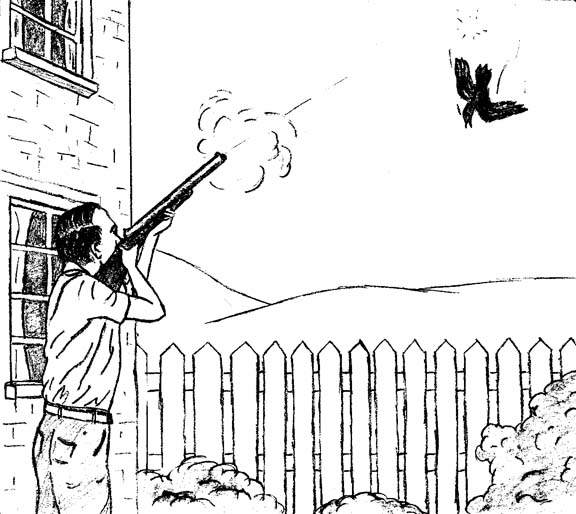
\includegraphics[width=0.95\columnwidth]{figures/exampleprompt2.jpg}\\
\hline
\textbf{Response (L1)} \\
\hline
The man killing the beard. (Arabic)\\
\hline
A man is shutting a bird. (Chinese) \\
\hline
A man is shooting a bird. (English) \\
\hline
The man shouted the bird. (Spanish)\\
\hline
\end{tabular}
\end{center}
\caption{Example item and responses}
\label{fig:example-picture}
\end{figure}

The PDT consists of 10 items (8 line drawings and 2 photographs\footnote{We have not observed substantial differences between responses for the drawings and the photographs.}) intended to elicit a single sentence
each; an example is given in Figure~\ref{fig:example-picture}. Participants
were asked to view the image and describe the action in past or present tense.
The data consist of responses from 53 informants (14 NSs, 39 NNSs),
for a total of 530 sentences, with the NNSs being intermediate and
upper-level adult English learners in an intensive English as a Second
Language program.  The distribution of first languages (L1s) is: 14
English, 16 Arabic, 7 Chinese, 2 Japanese, 4 Korean, 1 Kurdish, 1
Polish, 2 Portuguese, and 6 Spanish.

Responses were typed by the participants themselves, with spell checking disabled in some cases.  Even among the NNSs that used spell checking, a number of spelling errors resulted in real words. To address this, we use a spelling correction tool to obtain candidate spellings for each word, prune the candidates using word lists from the NS responses, recombine candidate spellings into candidate sentences, and evaluate these with a trigram language model (LM) to select the most likely intended response \citep{king:dickinson:14}.

Once the responses had been collected, the NNS responses were
annotated for correctness, with respect to the content of the picture.
The lead author marked spelling and meaning errors which prevent a
complete mapping to correct information
\citep[see][]{king:dickinson:13}.  On the one hand, minor misspellings
are counted as incorrect (e.g., \textit{The artiest is drawing a
\textbf{portret}}), while, on the other hand, the annotation does
not require distinguishing between between spelling and meaning
errors.  In the future, we plan on fine-tuning the annotation
criteria.

\section{Generalizing the Methods}
\label{sec:ranking}

The previous work assumed that the assessment of NNS responses
involves determining whether the gold standard (GS) contains the same
semantic triple that the NNS produced, i.e., whether a \textit{triple}
is \textit{covered} or \textit{non-covered}.  In such a situation the
GS need only be comprised of \textit{types} of semantic triples.  But
the GS is comprised of the small set of NS responses\md{I just noticed that I don't
think we ever said that GS=NS responses}\lk{nice catch---that explains the reviewer's confusion} and is thus
incomplete---meaning that exact matching is going to miss many cases,
and indeed in \citet{king:dickinson:13}, we note
that GS coverage is only at 50.8\%.  Additionally, relying on matching
of triples limits the utility of the method to specific semantic
requirements, namely transitive sentences.  By moving to bags of
dependencies and tallying the counts of (NS) responses in the GS, we
can move into a gradable, or ranking, approach to NNS responses.

We want to emphasize the degree to which a response conveys the same
meaning as the GS, necessitating an approach which can automatically
determine the importance of a piece of information in the GS.  We
break this down into how we represent the information
(section~\ref{sec:representation}) and then how we compare NNS
information to GS information (section~\ref{sec:scoring}), allowing us
to rank responses from least to most similar to the GS.\footnote{Although rankings often go from highest to lowest, we prioritize identifying problematic cases, so we rank accordingly.}  We also
discuss the handling of various other system parameters (section~\ref{sec:parameters}).

\subsection{Representation}
\label{sec:representation}

To overcome the limitations of an incomplete GS, we represent each
response as a list of \textit{terms} taken from the dependency parse
\citep{demarneffe:ea:06}, the terms referring to
%being either 
individual dependencies (i.e., relations between words).
%or individual words. 
This eliminates the complications of extracting semantic triples from
dependency parses, which could only handle a very restricted set of
grammatical forms and resulted in errors in 7--8\% of cases
\citep{king:dickinson:13}. Operating directly on individual
%words or
dependencies from the overall tree also means the system can allow for
``partial credit''; it distributes the matching over smaller,
overlapping pieces of information rather than a single, highly
specific triple.

Specifically, representations take one of five forms.  We first
tokenize and lemmatize the response to a list of lemmas that
represents the response.
The five term representations are then variations on dependencies. The
full form concatenates the label, head and dependent, as in
\texttt{subj\#boy\#kick}. We call this \textbf{ldh} (label, dependent,
head). The remaining four forms abstract over either the label, head
and/or dependent, as in \texttt{X\#boy\#kick}. We refer to these forms
as \textbf{xdh}, \textbf{lxh}, \textbf{ldx}, and \textbf{xdx}. 

The \param{xdx} model is on a par with treating the sentence as a bag
of lemmas, except that some function words not receiving parses (e.g.,
prepositions) are not included \citep[see][]{king:dickinson:13}.

In our current experiments, we test each of these term representations
separately, but we expect to ultimately make use of some weighted
combination. Future representations may also incorporate WordNet
relations or semantic role labeler output.

\subsection{Scoring Responses}
\label{sec:scoring}

Taking the term representations from the previous section, the next
task is to combine them in a way which ranks responses from least to
most appropriate.  Responses are scored with one of four approaches,
using one of two methods to \textbf{weight} response terms combined
with one of two methods to \textbf{compare} the weighted NNS terms
with the GS.

For weighting, we use either a simple frequency measure (\textbf{F})
or one based on \textbf{tf-idf} (\textbf{T})
\citep[][ch. 6]{manning-et-al:08}.  We explore tf-idf as a measure of
a term's importance with the hope that it is able to reduce the impact
of semantically unimportant terms---e.g., determiners like
\textit{the}, frequent in the GS, but unimportant for evaluating the
semantic contents of NNS responses---and to upweight terms which may
be salient but infrequent, e.g., only used in a handful of GS
sentences. For example, for an item depicting a man shooting a bird
(see Table~\ref{tab:i10responses-avgprec} and Figure~\ref{fig:example-picture}), of 14 GS responses, 12
described the subject as \textit{man}, one as \textit{he} and one as
\textit{hunter}. Since \textit{hunter} is infrequent in English, even
one instance in the GS should get upweighted via tf-idf, and indeed it
does. 
This is valuable, as numerous NNS responses use \textit{hunter}.

Calculating tf-idf relies on both \emph{term frequency} ($tf$) and
\emph{inverse document frequency} ($idf$).  Term frequency is simply
the raw count of an item, and for tf-idf of terms in the GS, we take
this as the frequency within the GS.  Inverse document frequency is
derived from some reference corpus, and it is based on the notion that
appearing in more documents makes a term less informative with respect
to distinguishing between documents.  The formula is in
(\ref{ex:tfidf}) for a term $t$, where $N$ is the number of documents
in the reference corpus, and $df_{t}$ is the number of documents
featuring the term ($idf_{t} = \log \frac{N}{df_{t}}$).  A term
appearing in fewer documents will thus obtain a higher $idf$ weight,
and this should readjust frequencies based on semantic importance.

\begin{exe}
\ex\label{ex:tfidf} $tfidf(t) = tf_{GS} \log \frac{N}{df_{t}}$
%, where $df_t = |\{d\in D, t \in d\}|$
\end{exe}

After counting/weighting, the frequencies are then either
\textbf{averaged} to yield a response score (\textbf{A}), or NNS term
weights and GS term weights are treated as vectors and the response
score is the \textbf{cosine distance} (\textbf{C}) between them.  This
yields:

%%former approach names: b = FA; m = IC (TC); c = FC; a = IA (TA)
\paragraph{Frequency Average (FA).} 
%This approach serves as our baseline. 
Within the GS, the frequency of each term is calculated. Each term in
the NNS response is then given a score equal to its frequency in the
GS; terms missing from the GS are scored zero. The response score is
the average of the term scores, with higher scores closer to the GS.

\paragraph{Tf-idf Average (TA).} This involves the exact same
averaging as with model FA, but now the terms in the GS are assigned
tf-idf weights before averaging.

\paragraph{Frequency Cosine (FC).} The frequency of each term is
calculated within the GS and (separately) within the NNS response. 
%\marginpar{\scriptsize{LK: above: "cosine distance (C)", so I changed "Comparison" (FC) to "Cosine". Good? I need to scan for other instances.}}
The term scores are then treated as vectors, and the response score is
the cosine distance between them, with lower scores being closer to
the GS.

\paragraph{Tf-idf Cosine (TC).} This involves the exact same
distance comparison as with model FC, but now the terms of both the GS
and NNS responses are assigned tf-idf weights before comparison.

\subsection{System Parameters}
\label{sec:parameters}

In addition to the four approaches, we have term representations and
two sets of parameters, listed below, to vary, resulting in a total of
60 settings for processing responses (see also
Table~\ref{tab:dist-ranked-parameters}). 

\paragraph{Term form.} As discussed in
section~\ref{sec:representation}, the terms can take one of five
representations: \param{ldh}, \param{xdh}, \param{lxh}, \param{ldx},
or \param{xdx}.
%\param{lemma}, \param{ldh}, \param{xdh}, \param{lxh}, \param{ldx}.

\paragraph{Scoring approach.} As discussed in
section~\ref{sec:scoring}, the NNS responses can be
compared with the GS via models \param{FA}, \param{TA}, \param{FC}, or \param{TC}.

\paragraph{Reference corpus.} The reference corpus for deriving tf-idf
scores can be either the Brown Corpus \citep{kucera:francis:67} or the
Wall Street Journal (WSJ) Corpus \citep{marcus-et-al:93}. These are
abbreviated as \param{B} and \param{W} in the results
below; \param{na} indicates the lack of a reference corpus, as this is
only relevant to approaches \param{TA} and
\param{TC}. The corpora are divided into as many documents as
originally distributed (\param{W}: 1640, \param{B}: 499). The WSJ is
larger, but Brown has the benefit of containing more balance in its
genres (vs. newstext only). Considering the narrative nature of PDT
responses, a reference corpus of narrative texts would be ideal, but
we choose manually parsed reference corpora as they are more reliable
than automatically parsed data.

\paragraph{NNS source.} Each response has an original version
(\param{NNSO}) and the output of a language model spelling corrector
%\texttt{+} module
(\param{NNSLM}) (see section~\ref{sec:data}).
% \citep{king:dickinson:14}. => cited in earlier section
%%%for now, let's hide this for anonymity's sake?

\subsection{Results}

\subsubsection{Evaluation metrics}
\label{sec:metrics}

We ran 60 response experiments, each with different system settings
(section~\ref{sec:parameters}). Within each experiment, we rank the 39
scored NNS responses from least to most similar to the GS.
%\md{Do we want to add something parenthetical like ``least coming first to model error detection''? (I can't think how to say it concisely.)} 
\md{Could/Should the footnote go into section 3?}
\lk{It could, but I kinda like it here}
For assessing these settings themselves, we rely on past annotation,
which counted unacceptable responses as errors (see
section~\ref{sec:data}).\footnote{The source of the error is also
labeled---stemming from NNS unintelligibility or a system error
(from spelling correction, parsing, or some downstream
component)---but we do not currently use this annotation.}  As the
lowest rank indicates the greatest distance from the GS, a good system
setting should ideally position the unacceptable responses among those
with the lowest rankings. Thus, we assign each error-containing
response a score equal to its rank, or, if necessary, the average rank
of responses sharing the same score.

In Table~\ref{tab:i10responses-avgprec}, an excerpt of sentence
responses is shown for one item, ranked from lowest to highest.  To
take one example, the third-ranked sentence, \textit{the man is hurting duck}, has a score of 0.996, and it is annotated as an error (1 in
the \textit{E} column).  Thus, the evaluation metric adds a score of 3
to the overall sum.  The sentence ranked 18, by contrast, is not an
error, and so nothing is added.  In the case of the top rank, two
responses with errors are tied, covering rank 1 and 2, so each adds a score of 1.5.

\begin{table}[htb!]
\begin{center}
\setlength{\tabcolsep}{0.3em}
\begin{tabular}{|r|c|l|r|r|}
\hline
\textit{R} & \textit{S} & Sentence & \textit{E} & \textit{V}\\
\hline
\hline
\multirow{2}{*}{1} & 1.000 & she is hurting. & 1 & 1.5 \\
& 1.000 & man mull bird & 1 & 1.5 \\
\hline
3 & 0.996 & the man is hurting duck. & 1 & 3.0 \\
4 & 0.990 & he is hurting the bird. & 1 & 3.0 \\
\hline
11 & 0.865 & the man is trying to hurt a bird & 1 & 11.0 \\
12 & 0.856 & a man hunted a bird. & 0 & 0.0 \\
\hline
17 & 0.775 & the bird not shot dead.  & 1 & 17.0 \\
18 & 0.706 & he shot at the bird & 0 & 0.0 \\
19 & 0.669 & a bird is shot by a un & 1 & 19.0 \\
20 & 0.646 & the old man shooting the birds & 0 & 0.0 \\
\hline
37 & 0.086 & the old man shot a bird. & 0 & 0.0 \\
38 & 0.084 & a old man shot a bird. & 0 & 0.0 \\
39 & 0.058 & a man shot a bird & 0 & 0.0 \\
\hline
\hline
\multicolumn{3}{|c|}{Total (Raw)} & 17 & 169 \\
\hline
\multicolumn{3}{|c|}{Average Precision} & \multicolumn{2}{c|}{0.75084} \\
\hline
\end{tabular}
\caption{Rankings for Item 10 from the best system setting (TC\_B\_NNSLM\_ldh) based on average precision scores. \textit{R}: rank; \textit{S}: sentence score; \textit{E}: error; \textit{V}: rank value. }
\label{tab:i10responses-avgprec}
\end{center}
\end{table}

The sum of these scores is taken as the \textbf{Raw} metric for that
experimental setting. In many cases, one version of a response
(\param{NNSO} or \param{NNSLM}) contains an error, but the other
version does not. Thus, for example, an \param{NNSO} experiment may
result in a higher error count than the \param{NNSLM} equivalent, and
in turn a higher Raw score.
In this sense, Raw scores emphasize error reduction and incorporate
item difficulty.

However, it is possible that the \param{NNSO} experiment, even with
its higher error count and Raw score, does a better job ranking the
responses in a way that separates good and erroneous ones. To account
for this, we also use \textbf{(mean) average precision ((M)AP)}
\citep[][ch. 8]{manning-et-al:08}, which emphasizes discriminatory
power.

For average precision (AP), one calculates the precision of error
detection at every point in the ranking, lowest to highest.  In
Table~\ref{tab:i10responses-avgprec}, for example, the precision for
the first cut-off (1.000) is 1.0, as two responses have been
identified, and both are errors ($\frac{2}{2}$). At the 11th- and
12-ranked response, precision is 1.0 ($\frac{11}{11}$) and 0.917
(=$\frac{11}{12}$), respectively, precision dropping when the item is
not an error.
AP averages over the precisions for all $m$ responses ($m=39$ for our
NNS data), as shown in (\ref{ex:ap}), with each response notated as
$R_k$.  Averaging over all 10 items results in the Mean AP (MAP).

\begin{exe}
\ex\label{ex:ap} $AP(item) = \frac{1}{m} \sum\limits_{k=1}^m
Precision(R_k)$
\end{exe}

As mentioned, the Raw metric emphasizes error reduction, as it
reflects not just performance on identifying errors, but also the
effect of the overall number of errors.  In this way, it may be useful
for predicting future system performance, an issue we explore in the
evaluation of clustering items (section~\ref{sec:clusteringresults}).
MAP, on the other hand, emphasizes finding the optimal separation
between errors and non-errors and is thus more of the focus in the
evaluation of the best system parameters next.

\subsubsection{Best system parameters} 

To start the search for the best system parameters, it may help to
continue our single example, in
Table~\ref{tab:i10responses-avgprec}. The best setting, as determined by the
Normalized metric, uses the tf-idf cosine (\param{TC}) approach with the Brown Corpus (\param{B}),
the spelling corrected response (\param{NNSLM}), and the full form of
the dependencies (\param{ldh}). It ranks highest because errors are
well separated from non-errors; the highest ranked of 17 total errors
is at rank 19.  Digging a bit deeper, we can see in this example how
the verb \textit{shoot} is common in all the highest-ranked cases shown
(\#37--39), but absent from all the lowest, showing both the effect of
the GS (as all NSs used \textit{shoot} to describe the action) and the
potential importance of even simple representations like lemmas.  In
this case, the \param{ldh} representation is best, likely because the
word \textit{shoot} is not only important by itself, but also in terms
of which words it relates to, and how it relates (e.g.,
\texttt{dobj\#bird\#shoot}).

\begin{table*}
\begin{center}
\begin{tabular}{|l|r||l|r||l|r||l|r|}
\hline
\multicolumn{2}{|c||}{Approach} & \multicolumn{2}{|c||}{Term Form} & \multicolumn{2}{|c||}{Ref. Corpus (TA/TC)} & \multicolumn{2}{|c|}{NNS Source} \\
\hline
\hline
0.51577 & TC & xdh & 0.51810 & Brown & 0.51534 & NNSLM & 0.51937 \\
\hline
0.50780 & FC & ldh & 0.51677 & WSJ & 0.50798 & NNSO & 0.49699 \\
\hline
0.50755 & TA & lxh & 0.51350 & & & & \\
\hline
0.49464 & FA & xdx & 0.49901 & & & & \\
\hline
& 	& ldx & 0.49352 &  &  &  & \\
\hline
\end{tabular}
\caption{Approaches and parameters ranked by mean average precision for all 10 PDT items.}
\label{tab:dist-ranked-parameters}
\end{center}
\end{table*}

Table~\ref{tab:all-dist-ranked-settings} shows the five best and five
worst system settings averaged across all 10 PDT items, as ranked by
MAP. Among the trends that pop out is a favoritism
towards \param{NNSLM} models (i.e., spelling correction). This is due
to the fact that higher numbers of errors inflate the MAP scores, and
somewhat counterintuitively, the spelling correction module introduces
more errors than it corrects, meaning there are more errors present
overall in the \param{NNSLM} responses than in the \param{NNSO}
responses.\footnote{Note that among the remaining parameter classes,
variation does not effect the number of errors.}

Another feature among the best settings is the inclusion of heads in the dependency representations. In fact, the top 17 ranked settings all include heads (\param{lxh}, \param{xdh}, \param{ldh}); \param{xdx} first enters the rankings at 18, and \param{xdx} and \param{ldx} are common among the worst performers. This is likely due to the salience of the verbs in these transitive sentences; they constitute the heads of the subjects and objects, in relatively short sentences with few dependencies.
Furthermore, the tf-idf weighted models dominate the rankings, especially \param{TC}. It is also clear that for our data tf-idf works best with the Brown Corpus (\param{B}).

\begin{table}[htb!]
\begin{center}
\begin{tabular}{|r|l|c|}
\hline
Rank & MAP & Settings \\
\hline
\hline
1 & 0.5534 & TC\_B\_NNSLM\_lxh \\
\hline
2 & 0.5445 & TA\_B\_NNSLM\_lxh \\
\hline
3 & 0.5435 & TC\_W\_NNSLM\_lxh \\
\hline
4 & 0.5422 & TC\_B\_NNSLM\_xdh \\
\hline
5 & 0.5368 & TC\_B\_NNSLM\_ldh \\
\hline
\hline
56 & 0.4816 & TA\_B\_NNSO\_xdx \\
\hline
57 & 0.4796 & FA\_na\_NNSLM\_ldx \\
\hline
58 & 0.4769 & FC\_na\_NNSO\_lxh \\
\hline
59 & 0.4721 & TA\_W\_NNSO\_xdx \\
\hline
60 & 0.4530 & FA\_na\_NNSO\_lxh \\
\hline
\end{tabular}
\caption{Based on Mean Average Precision, the five best and five worst settings across all 10 PDT items.}
\label{tab:all-dist-ranked-settings}
\end{center}
\end{table}

We also summarize the rankings for the individual parameter classes,
presented in Table~\ref{tab:dist-ranked-parameters}, confirming the
trends in Table~\ref{tab:all-dist-ranked-settings}. For a given
parameter, e.g., \param{ldh}, we averaged the experiment scores from
all settings including \param{ldh} across all 10 items. Notably, \param{TC} outperforms the other models, with \param{FC} and \param{TA} close behind (and nearly tied). Performance falls for the simplest model, \param{FA}, which was in fact intended as a baseline. With \param{TC}$>$\param{FC} and \param{TA}$>$\param{FA}, tf-idf weighting seems preferable to basic frequencies.

Again, the importance of including heads in dependencies is apparent here; the three dependency representations containing heads constitute the top three, with a sizable drop in performance for the remaining two forms (\param{xdx} and \param{ldx}). Moreover, given the content and narrative style of the PDT responses, it is unsurprising that the Brown Corpus serves as a better reference corpus than the WSJ Corpus for tf-idf. Finally, the \param{NNSLM} source significantly outperforms the \param{NNSO} source.

Despite the strength of these overall trends, variability
does exist among the best settings for different items, a point obscured
in the averages.  In Tables~\ref{tab:i01-dist-ranked-settings} and
\ref{tab:i05-dist-ranked-settings}, we present the best and worst
ranked settings for two of the least similar items, 1 and 5.
Their dissimilarity can be seen at a glance, simply from the range of
the AP scores (0.05--0.31 for item 1 vs. 0.52--0.81 for item 5), which
in itself reflects a differing number of erroneous responses (2 [\param{NNSO}]
or 6 [\param{NNSLM}] for item 1 vs. 23 or 24 for item 5).

For item 1, a drawing of a boy kicking a ball, we see considerable
variability in the best approach just within the top five settings:
all four approaches are in the top five.  Contrary to the overall
trends, we also see the \param{ldx} form---without any head
information---in the two best settings.  Note also that, even though
tf-idf weighting (\param{TA}/\param{TC}) is among the best settings, it is
consistently the worst setting, too.

For item 5 in Table~\ref{tab:i05-dist-ranked-settings}, a drawing of a
man raking leaves, the most noticeable difference is that
of \param{xdx} being among three of the top five settings.
We believe that part of the reason for
the superior performance of \param{xdx} (cf. lemmas), is that for this
item, all the NSs use the verb \textit{rake}, while none of the NNSs use this word.  For item 1 (the boy kicking a ball), there is lexical variation
for both NSs and NNSs.

\begin{table}[htb!]
\begin{center}
\begin{tabular}{|r|c|c|}
\hline
Rank & AP & Settings \\
\hline
\hline
1 & 0.30997 & TC\_B\_NNSLM\_ldx \\
\hline
2 & 0.30466 & TA\_B\_NNSLM\_ldx \\
\hline
3 & 0.30015 & TA\_B\_NNSLM\_xdh \\
\hline
4 & 0.29704 & FC\_na\_NNSLM\_xdh \\
\hline
5 & 0.29650 & FA\_na\_NNSLM\_ldh \\
\hline
\hline
56 & 0.06474 & TC\_B\_NNSO\_ldx \\
\hline
57 & 0.06174 & TC\_W\_NNSO\_ldx \\
\hline
58 & 0.06102 & TA\_W\_NNSO\_lxh \\
\hline
59 & 0.05603 & TA\_W\_NNSO\_xdx \\
\hline
60 & 0.05094 & TA\_W\_NNSO\_ldx \\
\hline
\end{tabular}
\caption{Based on Average Precision, the five best and five worst settings for item 1.}
\label{tab:i01-dist-ranked-settings}
\end{center}
\end{table}

\begin{table}[htb!]
\begin{center}
\begin{tabular}{|r|c|c|}
\hline
Rank & AP & Settings \\
\hline
\hline
1 & 0.80965 & FA\_na\_NNSLM\_xdx \\
\hline
2 & 0.80720 & TA\_B\_NNSLM\_lxh \\
\hline
3 & 0.80473 & TC\_B\_NNSLM\_lxh \\
\hline
4 & 0.79438 & TC\_B\_NNSLM\_xdx \\
\hline
5 & 0.78108 & TC\_W\_NNSLM\_xdx \\
\hline
\hline 
56 & 0.56495 & FC\_na\_NNSO\_xdh \\
\hline
57 & 0.56414 & TC\_B\_NNSO\_lxh \\
\hline
58 & 0.55890 & TC\_W\_NNSO\_lxh \\
\hline
59 & 0.54506 & FC\_na\_NNSO\_lxh \\
\hline
60 & 0.52013 & FA\_na\_NNSO\_lxh \\
\hline
\end{tabular}
\caption{Based on Average Precision, the five best and five worst settings for item 5.}
%%LK: fixed 4/6 pm.
\label{tab:i05-dist-ranked-settings}
\end{center}
\end{table}

These types of differences---for these items and others---
lead us to explore the clustering of item patterns, in order to
leverage these differences and automatically choose the optimal
settings for new items; we turn to this next.

\section{Clustering}
\label{sec:clustering}

Given the variability of NS and NNS responses, and the possible
correlation with different system parameters, we have begun exploring
connections by clustering the different items.  The clustering uses,
for one set, \emph{response features}, i.e., features observable from
the responses, and, separately, \emph{performance features}, i.e., the
performance of different system settings on the responses.

Although the work is very exploratory, our goal is to get a handle on
learner variability for different items and explore correlations
between response and performance clusters.

\subsection{Response Clustering}

We cluster the 10 PDT items using simple features taken from the
responses themselves. Specifically, we use various combinations of
type counts, token counts, and type-to-token ratios for each term form
(\param{ldh}, \param{xdh}, \param{lxh}, \param{ldx}, \param{xdx}),
taken from each response source (GS, \param{NNSO}, \param{NNSLM}).

\subsection{Performance Clustering}

From the system output, we cluster items using per-item Raw 
scores for various settings. That is, for each of the 10 items, we
calculate an average error score for each approach
(\param{FA}, \param{TA}, \param{FC}, \param{TC}), each term form
(\param{ldh}, \param{xdh}, \param{lxh}, \param{ldx}, \param{xdx}),
each reference corpus (\param{B}, \param{W}), and each
response source (\param{NNSO}, \param{NNSLM}). 
As mentioned in section~\ref{sec:metrics}, Raw scores should account for the number of
errors produced by NNSs for each item, which should 
correlate with future system performance.

\subsection{Results}
\label{sec:clusteringresults}

Although there is noise in some experiments, some patterns do seem to
emerge in many of the clusterings; we present some of the most common
patterns here.

Figure~\ref{fig:response-clusters} shows a clustering based on
response features that shares some characteristics with
Figure~\ref{fig:parameter-clusters}, a clustering based on performance
features. (Note that clustering heights are not to scale.)  In both
examples, items 5 and 9 form a cluster attaching to the root. These
are described in the GS as \textit{A man is raking leaves} and
\textit{Two boys are rowing a boat}. These were also the two most
difficult items for NNSs. While other items involved common verbs like
\textit{kick}, \textit{paint} and \textit{cut}, the actions depicted
in these items were more specific and required words outside the
vocabulary of many participants. For example, while all 14 NSs used
either \textit{row} or \textit{paddle}, only five of 39 NNSs used
these verbs; the rest used verbs like \textit{boat}, \textit{sail},
\textit{sit}, \textit{play} or \textit{ride}.

\begin{figure}
\begin{center}
\begin{tikzpicture}[sloped]
\node (5) at (-7.5,0) {5};
\node (9) at (-6.9,0) {9};
\node (1) at (-6.2,0) {1};
\node (4) at (-5.5,0) {4};
\node (6) at (-4.7,0) {6};
\node (2) at (-4.0,0) {2};
\node (8) at (-3.2,0) {8};
\node (10) at (-2.6,0) {10};
\node (3) at (-1.8,0) {3};
\node (7) at (-1.1,0) {7};
\node (59) at (-7.2,0.7) {};
\node (14) at (-5.9,0.7) {};
\node (28) at (-3.5,0.7) {};
\node (37) at (-1.5,0.7) {};
\node (1037) at (-2.3,1) {};
\node (281037) at (-2.9,1.3) {};
\node (6281037) at (-3.6,1.7) {};
\node (146281037) at (-4.9,2.1) {};
\node (59146281037) at (-6.4,2.5) {};
\draw  (5)  |- (59.center);
\draw  (9)  |- (59.center);
\draw  (1)  |- (14.center);
\draw  (4)  |- (14.center);
\draw  (2)  |- (28.center);
\draw  (8)  |- (28.center);
\draw  (3)  |- (37.center);
\draw  (7)  |- (37.center);
\draw (10) |- (1037.center);
\draw (37) |- (1037.center);
\draw (1037) |- (281037.center);
\draw (28) |- (281037.center);
\draw (6) |- (6281037.center);
\draw (281037) |- (6281037.center);
\draw (14) |- (146281037.center);
\draw (6281037) |- (146281037.center);
\draw (59) |- (59146281037.center);
\draw (146281037) |- (59146281037.center);
\end{tikzpicture}
\end{center}
\caption{PDT items clustered by type and token counts of all NS, NNSO and NNSLM responses.} 
%%duh?%%(Heights not to scale.)}
\label{fig:response-clusters}
\end{figure}

\begin{figure}
\begin{center}
\begin{tikzpicture}[sloped]
\node (5) at (-7.5,0) {5};
\node (9) at (-6.9,0) {9};
\node (3) at (-6.2,0) {8};
\node (8) at (-5.5,0) {3};
\node (2) at (-4.7,0) {2};
\node (10) at (-4.0,0) {10};
\node (1) at (-3.2,0) {1};
\node (4) at (-2.6,0) {4};
\node (6) at (-1.8,0) {6};
\node (7) at (-1.1,0) {7};
\node (59) at (-7.2,.8) {};
\node (210) at (-4.3,.7) {};
\node (14) at (-2.9,.7) {};
\node (67) at (-1.5,.7) {};
\node (8210) at (-4.9,1.0) {};
\node (38210) at (-5.7,1.3) {};
\node (1467) at (-2.2,1.4) {};
\node (382101467) at (-4,2) {};
\node (all) at (-5,2.5) {};
\draw  (5) |- (59.center);
\draw  (9) |- (59.center);
\draw  (2) |- (210.center);
\draw  (10) |- (210.center);
\draw  (1) |- (14.center);
\draw  (4) |- (14.center);
\draw  (6) |- (67.center);
\draw  (7) |- (67.center);
\draw  (8) |- (8210.center);
\draw  (210) |- (8210.center);
\draw  (8210) |- (38210.center);
\draw  (3) |- (38210.center);
\draw  (14) |- (1467.center);
\draw  (67) |- (1467.center);
\draw  (38210) |- (382101467.center);
\draw  (1467)  |- (382101467.center);
\draw  (59)  |- (all.center);
\draw  (382101467)  |- (all.center);
\end{tikzpicture}
\end{center}
\caption{PDT items clustered by parameter performance.} 
%%duh?%%(Heights not to scale.)}
\label{fig:parameter-clusters}
\end{figure}

Items 1 and 4 also appear as a cluster in both cases. In GS examples,
these are described as \textit{The boy is kicking a ball} and
\textit{A man is reading a newspaper}. The images portray actions that
language learners often learn in beginner courses, and in fact, these
were the easiest items for NNSs. The simple actions and objects mean
that both token counts and type counts are relatively low. \md{Just to make sure: are these still the right parameters that perform highly?}\lk{I changed it slightly; these are best, but the trend isn't very strong via MAP. the trends are different via Raw, (and stronger, hence the cluster!) but I don't think we want to go into that, given that we present the MAP for item 1 in Table 4} With regard
to feature performance, for both items the same parameters perform
highly (\param{TC}/\param{TA}, \param{ldx}/\param{ldh}/\param{xdh}), suggesting that a future item
which clusters with these two would benefit from the same processing.

\section{Summary and Outlook}

We have investigated ways to reason about learner meaning in cases
where the set of correct meanings is incomplete, namely in the
case of picture description tasks (PDTs).  Specifically, we have
explored different models of representing and scoring NNS responses to
a picture---different linguistic representations, term weighting
schemes, reference corpora, and use of spelling correction---in order
to automatically determine the relevant parts of an image from a set
of NS responses.  In more exploratory work, we have also examined the
variability in both NS and NNS responses, and how different system
parameters correlate with the variability.  

Already, the results are providing insight for future system
development, data collection, and investigations into learner
language.  A big next step of the work is to collect more data, and
examining the variability in the NS/NNS data has provided feedback on
the types of new data to gather, to better ensure a wide range of
behavior from NNSs.  Getting a range of items, with different sentence
types and variability in responses, will help us properly find our
envisioned sweet spot of semantic analysis.  In that vein, we plan on
exploring more parameters (e.g., semantic role information) and
holding out data to better gauge the impact of clustering a new item
with the existing items and selecting the processing parameters on
that basis.

%%%% END material from BEA 2016 %%%%
